\section{学習する場所付近の反射強度}

  学習フェーズで使用する場所を\figref{Fig:RobotGuidance_exp3_foyer}に示す.ここは,千葉工業大学津田沼キャンパス2号館3階のホワイエと呼ばれる場所であり,中にはガラスや自動販売機が存在する.それぞれに対して反射強度を計測するのは大変なので,ホワイエをランダムに250秒間歩き回ることでデータを収集した.
  計測した結果を\figref{Fig:Histogram of reflection intensity of foyer}に示す.平均値は約2102であり,分散は約676261であった.

\vspace{0.2cm}

  \begin{figure}[h]
    \centering
    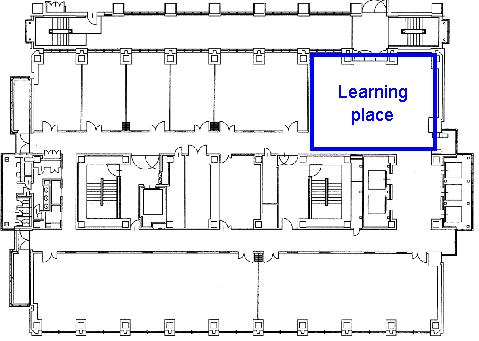
\includegraphics[width=7cm] {images/pdf/RobotGuidance_exp3_foyer}
    \captionsetup{justification=raggedright} % キャプションを左寄せに
    \caption{Measure the reflection intensity of foyer}
    \label{Fig:RobotGuidance_exp3_foyer}
  \end{figure}

  \vspace{-0.5cm}

  \begin{figure}[h]
    \centering
    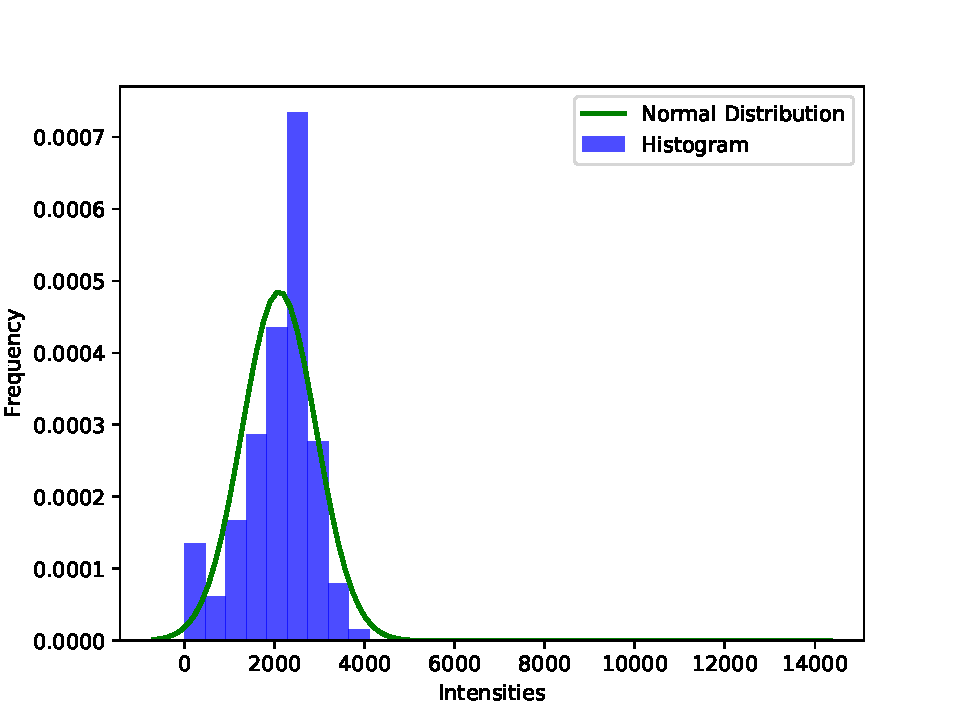
\includegraphics[keepaspectratio, scale=0.55] {images/pdf/RobotGuidance_plot_reflection_intensities_of_foyer}
    \captionsetup{justification=raggedright} % キャプションを左寄せに
    \caption{Histogram of reflection intensity of foyer}
    \label{Fig:Histogram of reflection intensity of foyer}
  \end{figure}

\newpage